
\chapter{Introduction}
\section{What are fake news?}
\subsection{Definition}
\paragraph{} Fake news have quickly become a society problem, being used to propagate false or rumorus informations in order to change behaviors of peoples. Before stating to work on detecting fake news, it is needed to first understand what they are. It have been show that propagation of fake news have had a non negligable influence of 2016 US presidential elections\cite{Allcott2017}. A few facts on fake news in the United States: 

\begin{itemize}
	\item $62\%$ of US citizen get there news for social medias\cite{gottfried2016news}
	\item Fake news had more share on facebook than mainstream news\cite{silverman2016teens}.
\end{itemize}

Fake news have also been used in order to influence the referendum in the United Kingdom for the "Brexit".

%TODO: Define fake news
%TODO: Expliquer les differentes méthodes de détection de fake news dans le paper Fake News Detection on Social Media: A Data Mining Perspective 1708.01967v3.pdf
\paragraph{}There are two aspects of fake news detection that need to be taken into account according to Shu et al\cite{shu2017fake}. The first is characterization or what are fake news and the second is detection. In order to build detection models, it is need to start by charaterization, indeed, it is need to understand what are fake news before trying to detect them. 
\paragraph{}
Fake news definition is made of two part: authenticity and intent. Authenticity means that fake news content fale information that can be verified as such, which means that concpiracy theory is not included in fake news as there are difficult to be proven true or false in most cases. The second part, intent, means that the false information have been written with the goal of missleading the reader. 


\begin{figure}
	\centering
	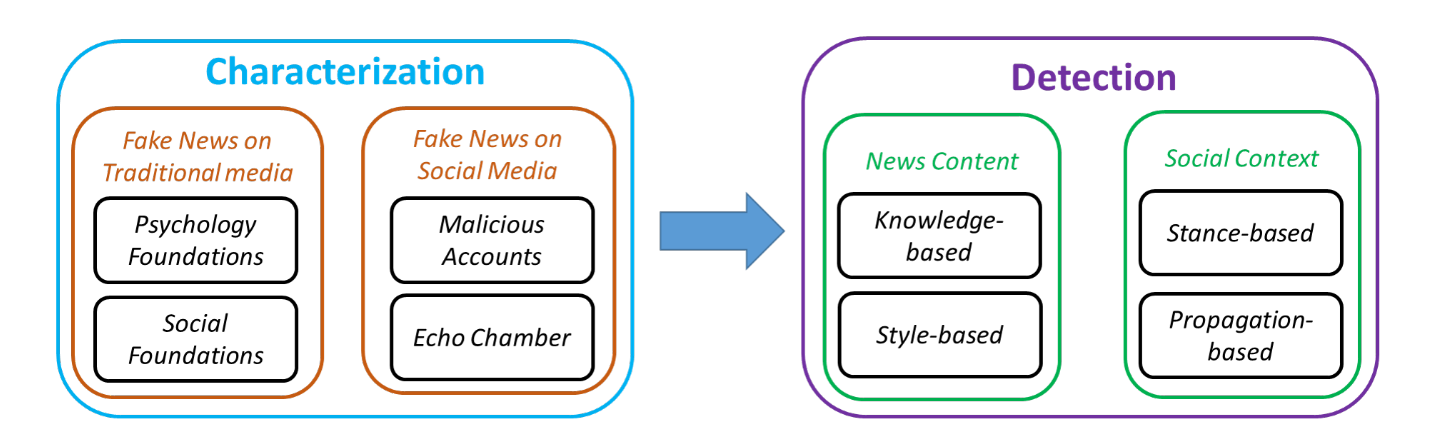
\includegraphics[width=0.8\textwidth]{chapter/images/introduction/characterization.png}
	\caption{Fake news on social media: from characterization to detection.\cite{shu2017fake}}
	\label{fig:intro:characterization}
\end{figure}

\subsection{Fake News Characterization}
\newtheorem{def:fake_news}{Definition}

\begin{def:fake_news}
Fake news is a news article that is intentionally and verifiably false
\end{def:fake_news}

The part of the definition introducing the intent of missleading the reader automaticaly discard satire news medias, that is why this works will focus on the first part, the fact that the piece of information is verifiably false or true. Indded, even if satire news medias does not have the intent to misslead the readers, not all of them have the ability of making criticisme and not taking it to the first degree. On the other hand, in the case of political media, even if it clearly try to influence the consumer, verifying the authenticity of there claims is usualy harder as, in most of the cases, openly lies. 

\section{Feature Extraction} \label{intro:feature_extract}
\subsection{News Content Features}
\paragraph{} Now that fake news have been defined and the target have been set, it is needed to analize what features can be used in order to classify fake news. Starting by looking at news content, it can be seen that it is made of four principal raw components: 
\begin{itemize}
	\item \textbf{Source}: Where does the news come from, who wrote it, is this source reliable or not.
	\item \textbf{Headline}: Short summary of the news content that try to attract the reader.
	\item \textbf{Body Text}: The actual text content of the news.
	\item \textbf{Image/Video}: Usualy, textual information is agremented with visual information such as images, videos or audio.  
\end{itemize}

\paragraph{} Features will be extracted from these four basic components, with the mains features being linguistic-based and visual-based. 
As explained before, fake news are used to influence the consumer, and in order to do that, they often use a specific language in order to attract the readers. On the other hand, non fake news will mostly stick to a different language register, being more formal. This are linguistic-based features, to which can be added lexical features such as total number of words, frequency of large words or unique words. 

The second features that need to be taken into account are visual features. Indeed, modified images are often used to add more weight to the textual information. For example, the \textbf{Figure \ref{fig:intro:deforestation}} is supposed to show the progress of deforestation, but the two images are acutaly from the same original one, and in addition the WWF logo make it looks like to be from a trusted source. 

\begin{figure*}
	\centering
	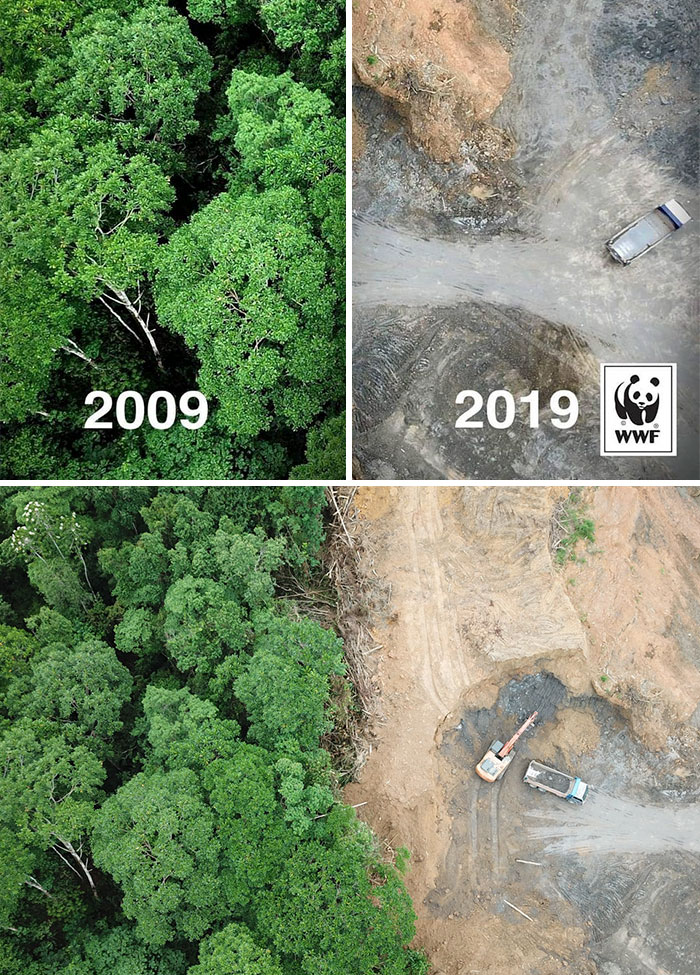
\includegraphics[width=0.8\textwidth]{chapter/images/introduction/fake-news-photos-viral-photoshop-8-5c6fe61f88240__700}
	\caption{The two images provided to show deforestation between two date are from the same image taken at the same time.}
	\label{fig:intro:deforestation}
\end{figure*}

\subsection{Social Context Features}
\paragraph{} In the context of news sharing on social medias, multiples aspect can be taken into account, such as user aspect, post aspect and group aspect. For instance, it is possible to analyize the behavior of specific users and use their metadata in order to find if a user is at risk of trusting or sharing false information. For instance, those metadata can be its center of intereset, its number of followers, or anything that relates to it. 

\paragraph{} Post-based aspect is in a sense similar to user based: it can use post metadata in order to provide usefull informations, but in addition to metadata, the actual content can be used. It is also possible to extract features from the content using latent Dirichlet allocation (LDA)\cite{blei2003latent}.

\section{News Content Models} \label{intro:models}
\subsection{Knowledge-based models}:
Now that the differents kinds of features available for the news have been defined, it is possible to start to explain what kind of models can be built using these features. The first models that relates to the news content is based on knowledge: the goal of this model is to check the truthfulness of the news content and can be acheived in tree differents way (or a mixture of them):

\begin{itemize}
	\item \textbf{Expert-oriented}: relies on expert, such as journalist or scientist, to asses the news content.
	\item \textbf{Crowdsourcing-oriented}: relies on the wisdom of crowd that says that if a suficiently large amount of persons says that something is false or true then it should be.
	\item \textbf{Computational-oriented}: relies on automatic fact checking, that could be based on external resources shuch as DBpedia.
\end{itemize}

These methods all have pros and cons, hiring expert might be constly, and expert are limited in number and might not be able to treat all the news that are produced. In the case of crowdsourcing it can easily be fooled if enought bad annotators breaks the system and automatic fact checking might not have the necessary accuracy.

\paragraph{Style-based model}: As explained earlier, fake news usualy tries to influence consumier behavior, and thus generaly use a specific style in order to play on the emotion. These methods are called deception-oriented stylometric methods.

The second method is called objectivity-oriented approaches and tries to capture the objectivity of the texts or headlines. These kind of style is mostly used by partisan article or yellow-journalism, that is, website that relies on eye-catching headline without reporting any useful information. An example of these kind of headline could be:
	\begin{quote}You will never beleive what he did !!!!!!\end{quote}
\paragraph{} This kind of headline plays on the curiosity of the reader that would click to read the news.

\subsection{Social Context Models}
\paragraph{} The last features that have not been used yet are social media features. There are two approaches to use these features: stance-based and propagation-based. 

\paragraph{Stence-based} approaches use implicit or explicit representation. For instance, explicit representation might be positive or negative votes on social medias. Implicit representation need to be extracted from the post itself. 

\paragraph{Propagation-based} approaches use features related to sharing such as the number of retweet on twitter. 

\section{Datasets} \label{intro:dataset}
\subsection{Fake News Corpus}
\paragraph{}
This works uses multiples corpus in order to train and test different models. The main corpus used for training is called Fake News Corpus\cite{Szpakowski}. This corpus have been automatically crawled using \url{opensources.co} labels. In other words, domains have been labeled with one or more labels in \begin{itemize}
	\item Fake News
	\item Satire
	\item Extreme Bias
	\item Conspiracy Theory
	\item Junk Science
	\item Hate News
	\item Clickbait
	\item Proceed With Caution
	\item Political
	\item Credible
\end{itemize}
\paragraph{}
These annotations have been provided by crowdsourcing, which means that they might not be exactly accurate, but are expected to be close to the reality. Because this works focus on fake news detection against reliable news, only the news labels as fake and credible have been used. 

\textbf{TODO: Expliquer comment le dataset a été nettoyé et mis dans une base de données afin d'augmenter les performances. }

\subsection{Fake News Net}
\paragraph{}
The second dataset used is fake news net\cite{shu2018fakenewsnet,shu2017exploiting,shu2017fake}. This corpus is made of news from two different sources, PolitiFact and GossipCop. An older version also provide news from BuzzFeed. News are categorized in two classes: fake and non fake. Being quite smaller than fake news corpus, this dataset will be used as a test dataset. 

\subsection{Liar, Liar Pants on Fire}
\paragraph{}
The third and last dataset is \textbf{Liar, Liar Pants on Fire} dataset\cite{Wang2017}, which is a collection of twelve thousand small sentences collected from various sources and hand labeled. They are devided in six classes:
\begin{itemize}
	\item pants-fire
	\item false
	\item barely-true
	\item half-true
	\item mostly-true
	\item true
\end{itemize} 
\paragraph{}
This set will be used a second test set. Because in this case there are six classes againt two in the other cases, a threshould should be used in order to fix which one will be concidered as true or false. 
\paragraph{}
It should be noted that this one differ from the two other dataset is it is composed only on short sentences, and thus it should not be expected to have very good results on this dataset for models trained on Fake News Corpus which is made of full texts. 

\section{State of the Art}
\section{Conclusion}
\paragraph{} As it have been show in \textbf{Section \ref{intro:feature_extract}} and \textbf{Section \ref{intro:models}} mutliples approaches can be used in order to extract features and use them in models. This works focus on textual news content features. Indeed, other features related to social medias are difficult to aquire. For example, users information are difficult to obtain on Facebook, as well as post information. In addition, the different datasets that have been presented at \textbf{Section \ref{intro:dataset}} does not provides any other information than textual ones. 

\paragraph{} Looking at \textbf{Figure \ref{fig:intro:features}} it can be seen that the main focus will be made on unsupervised and supervised learning models using textual news content. It should be noted that machine learning models usualy comes with a trade-off between precision and recall and thus that a model which is very good at detected fake news might have a high false positive rate as opposite to a model with a low false positive rate which might not be good at detecting them. This cause ethical questions such as automatic censorship that will not be discused here. 

\begin{figure*}
	\centering
	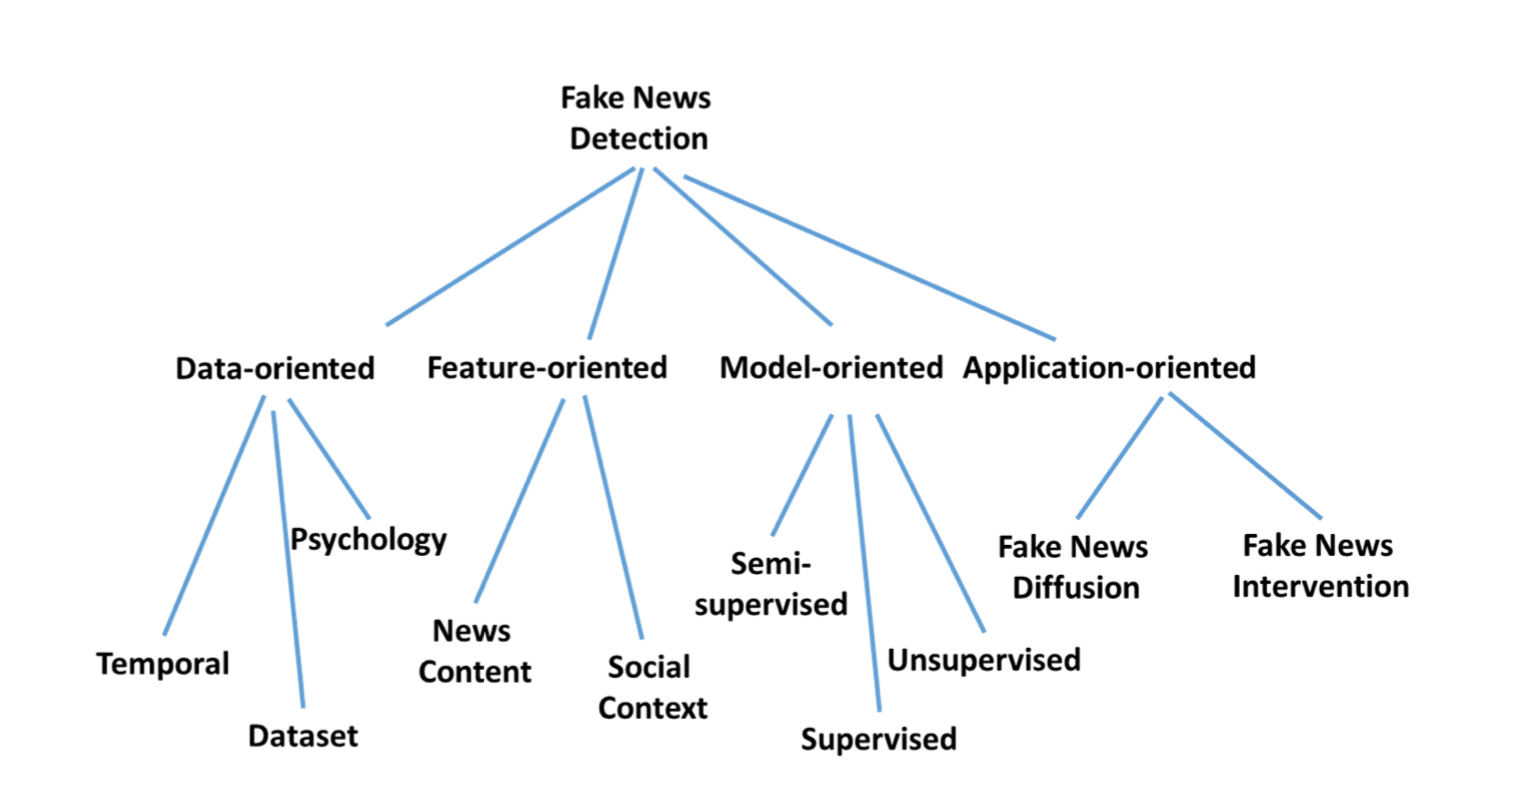
\includegraphics[width=0.8\textwidth]{chapter/images/introduction/features}
	\caption{Differents approaches to fake news detection.}
	\label{fig:intro:features}
\end{figure*}